\documentclass[11pt, a4paper]{article}

\usepackage{graphicx}
\usepackage[a4paper,top=3cm,bottom=2cm,left=2cm,right=2cm,marginparwidth=1.75cm]{geometry}
\usepackage[english]{babel}
\usepackage[utf8x]{inputenc}
\usepackage{subfig}
\usepackage{amsmath}
\usepackage{amssymb}

\graphicspath{ {./images} }
\newcommand*{\qed}{\hfill\ensuremath{\quad\square}}%
\newcommand*{\rad}{\ensuremath{\,\text{rad}}}
\newcommand*{\Rea}{\ensuremath{\text{Re}}}
\newcommand*{\Ima}{\ensuremath{\text{Im}}}
\newcommand*{\R}{\ensuremath{\mathbb{R}}}
\newcommand*{\C}{\ensuremath{\mathbb{C}}}

\makeatletter
\renewcommand*\env@matrix[1][*\c@MaxMatrixCols c]{%
  \hskip -\arraycolsep
  \let\@ifnextchar\new@ifnextchar
  \array{#1}}
\makeatother

\newtheorem{theorem}{Theorem}

%------------------------------------------------
%Templates for images and figures
% \begin{figure}[h]
%   \centering
%   \subfloat[caption 1]{{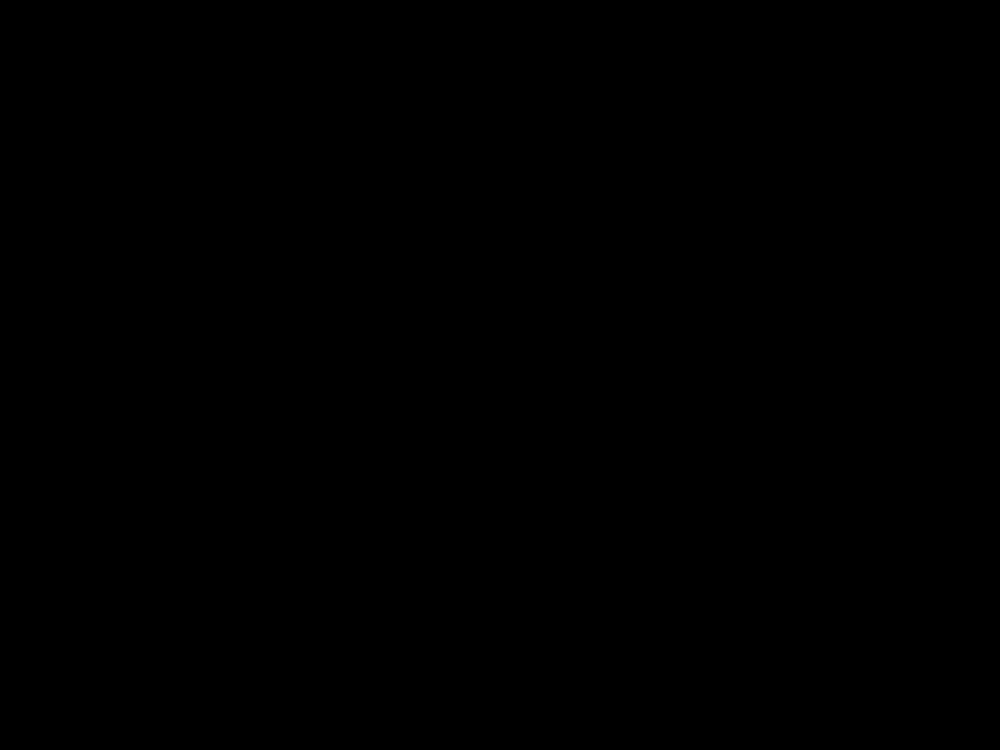
\includegraphics[width=30mm]{images/placeholder.png}}}%
%   \qquad
%   \subfloat[caption 2]{{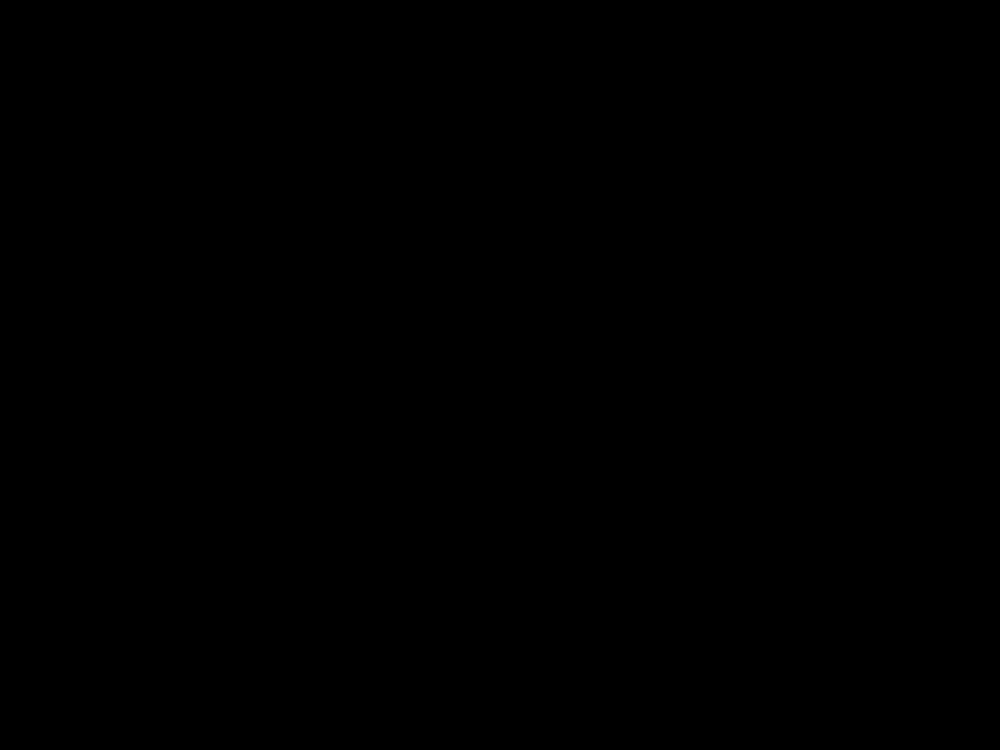
\includegraphics[width=30mm]{images/placeholder.png}}}%
%   \caption{Description}
% \end{figure}

% \begin{figure}[h]
%   \centerline{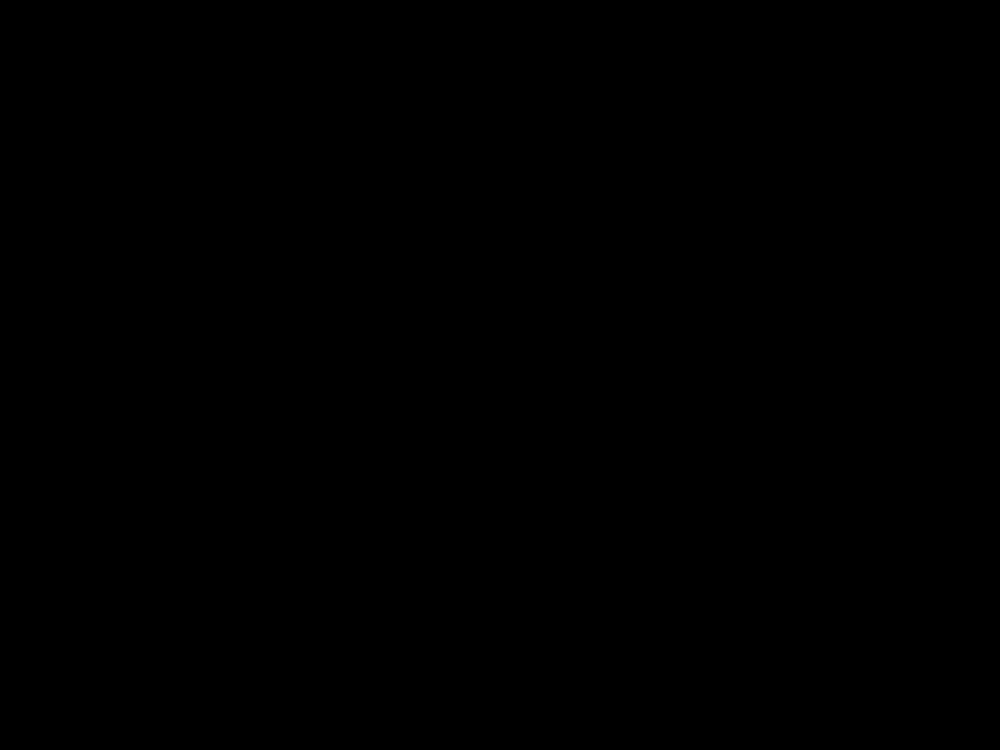
\includegraphics[width=50mm]{images/placeholder.png}}
%   \caption{Description}
% \end{figure}
%-----------------------------------------------

\begin{document}
\setcounter{equation}{0}
\setcounter{section}{4}
\section{Linear Algebra 2 Lecture 5: Complex eigenvalues (05/05/2020)}


\subsection{Properties of complex numbers}
Recall that complex numbers generally have the form:
\begin{equation}
  z = \alpha + \beta i
\end{equation}
Complex numbers have the following properties and iedentities:
\begin{itemize}
  \item $\Rea(z) = \alpha$
  \item $\Ima(z) = \beta$
  \item $\bar{z} = \alpha - \beta i$
  \item $z = r e^{i\theta}$
  \item $|z| = r =\sqrt{\alpha^2 + \beta^2}$
  \item $\text{arg}(z) = \arctan \left(\frac{\beta}{\alpha} \right)$
  \item $\frac{1}{i} = -i$
\end{itemize}
The entries of a vector or matrix may very well be complex. All the conventional rules of Gaussian elemination still apply but it becomes very very easy to make a ton of little mistakes. Thus in general it is prefferable to work with matrix with only real entries where possible.\\
Vectors can also be complex. In that case they usually take a form very similar to how complex numbers generally look:
\begin{equation}
  \vec{z} = \vec{\alpha} + \vec{\beta}i \in \C^n \quad \vec{\alpha},\, \vec{\beta} \in \R^n
\end{equation}
The real part of the vector $\vec{z}$ will be the vector $\Rea(\vec{z}) = \vec{\alpha}$. The imaginary part of the vector $\vec{z}$ will be the vector $\Ima(\vec{z}) = \vec{\beta}$. The complex conjugate vector of $\vec{z}$ is $\bar{\vec{z}} = \vec{\alpha} - \vec{\beta}i \in \C^n$


\subsection{Matrices with complex eigenvalues}
Consider the following matrix:
\begin{equation*}
  A = 
  \begin{bmatrix}
    2 & -1\\
    4 & 2\\
  \end{bmatrix}
\end{equation*}
When we try to find the eigenvalues of this matrix using the following identity: $A\vec{x} = \lambda \vec{x} \Rightarrow (A-\lambda I)\vec{x} = \vec{0}$ and solving for the determinant of $A-\lambda I$ we get the following characteristic polynomial:
\begin{equation*}
  (2 - \lambda)^2 + 4 = 0
\end{equation*}
Solving for the 2 eigenvalues $\lambda$ we find that the eigenvalues of this matrix are $\lambda_1 = 2 - 2i$ and $\lambda_2 = 2 + 2i$. Note that this pair of eigenvalues are eachothers complex conjugate. In other words: $\lambda_2 = \bar{\lambda}_1$. This idea applies to all complex eigenvalues of matrices and even extends to eigenvectors which will be shown later. If you found some complex eigenvalues it's complex conjugate will also be an eigenvalue. Using the eigenvalue $\lambda_2$ to find it's eigenvector we are left with:
\begin{equation*}
  (A-\lambda I)\vec{x} = \vec{0} \Rightarrow 
  \begin{bmatrix}[cc|c]
    -2i & -1  & 0\\
    4   & -2i & 0\\
  \end{bmatrix}
  \sim
  \begin{bmatrix}[cc|c]
    1   & -\frac{i}{2}  & 0\\
    0   & 0             & 0\\
  \end{bmatrix}
\end{equation*}
Which leaves us with the eigenvector $\vec{v} = \begin{bmatrix} \frac{i}{2} \\ 1\\ \end{bmatrix}$. This vector will then form the basis of the (complex) eigenspace $E_{2 + 2i} = \text{Span}\{ \vec{v} \}$.

Since we know that eigenvalues come in pairs we can assert the follwing: Let $A$ be an $n \times n$ matrix with only real entries. Let $\vec{x} \in \C^n$, let $\lambda$ be a complex eigenvalue.
\begin{equation*}
  A\vec{x} = \lambda \vec{x}
\end{equation*}
When we take the complex conjugate on both sides of the equation we end up with:
\begin{equation*}
  \bar{A}\bar{\vec{x}} = \bar{\lambda}{\bar{\vec{x}}}
\end{equation*}
Since we defined $A$ to only have real entries we know that it is it's own complex conjugate. Thus $\bar{A} = A$. The expression then reduces to:
\begin{equation}
  A \bar{\vec{x}} = \bar{\lambda}\bar{\vec{x}}
\end{equation}
Which directly implies that for each complex eigenvalue of $\lambda$ there is a corresponing complex conjugate $\bar{\lambda}$, and for each eigenvector $\vec{x}$ corresponding to $\lambda$ there is a complex conjugate of said eigenvector corresponding to the eigenvalue $\bar{\lambda}$.\\
Or in other words: if $A$ is an $n \times n$ matrix with only real elements and $\vec{v}$ is an eigenvector of $A$ with the corresponding eigenvalue $\lambda$ then $\bar{\vec{v}}$ is also an eigenvector of $A$ with the corresponding eigenvalue $\bar{\lambda}$.


\subsection{Computational shortcut for a $2 \times 2$ matrix with complex eigenvalues}
Recall the matrix $2 \times 2$ matrix from the previous example. Notice how Gaussian elemination results in a row of zeros. This is no accident and in fact makes finding eigenvectors of $2 \times 2$ matrices much easier. Since we know that the equation $(A - \lambda I)\vec{x} = \vec{0}$ must have a non-trivial solution. If the solution was in fact a trivial solution we can assert that $\lambda$ is not in fact a proper eigenvalue of the matrix. Thus when doing row-reduction on a $2 \times 2$ matrix we will ALWAYS get a row of zeros. This makes finding eigenvectors much easier since we can just set one row to all zero entries and solve for the free variable.


\subsection{Scale-Rotation matrices}
let $A = \begin{bmatrix} \alpha & -\beta\\ \beta & \alpha\\ \end{bmatrix}$ where $\alpha\,,\beta \in \R$. Then $A$ is a scale-rotaion matrix which scales space by a factor $r = |\alpha + \beta i|$ and rotates by an angle $\theta = \text{arg}(\alpha + \beta i)$. Since we can express complex numbers in polar coordinates as follows:
\begin{gather*}
  \alpha = r\cos(\theta)\\
  \beta = r\sin(\theta)
\end{gather*} 
Using this identity to rewrite the matrix $A$ we get the follwing:
\begin{equation}
  A =
  \begin{bmatrix}
    r\cos(\theta) & -r\sin(\theta)\\
    r\sin(\theta) & r\cos(\theta)\\
  \end{bmatrix}
  = r \cdot
  \begin{bmatrix}
    \cos(\theta) & -\sin(\theta)\\
    \sin(\theta) & \cos(\theta)\\
  \end{bmatrix}
\end{equation}
Which is nothing but the standard matrix for a rotation of space by an angle of $\theta$ but scaled by a factor of $r$. We are interested in scale-rotation matrices because, much like diagonal matrices, it's very easy to find high powers of such a matrix. This is because of the following relation:
\begin{equation*}
  A^n = \left( r \cdot
  \begin{bmatrix}
    \cos(\theta) & -\sin(\theta)\\
    \sin(\theta) & \cos(\theta)\\
  \end{bmatrix}
  \right)^n
  =
  r^n \cdot
  \begin{bmatrix}
    \cos(\theta) & -\sin(\theta)\\
    \sin(\theta) & \cos(\theta)\\
  \end{bmatrix}^n
\end{equation*}
Since rotating space $n$ times is exactly the same as rotating space in one go by the angle $n\theta$ we get the follwing:
\begin{equation}
  A^n =
  r^n \cdot
  \begin{bmatrix}
    \cos(n \theta) & -\sin(n \theta)\\
    \sin(n \theta) & \cos(n \theta)\\
  \end{bmatrix}
\end{equation}
Scale-rotation matrices can be used in a similarity transformation for a matrix $A$ with complex eigenvalues:
\begin{equation}
  A = PCP^{-1}
\end{equation}
Where $P$ is an invertible matrix and $C$ is some scale-rotation matrix. This allows us to easily find high powers of the matrix $A$ using the scale-rotation matrix $C$. Since this leaves us with an $P^{-1}P$ term which is nothing but the identity matrix we can create the following expression:
\begin{equation}
  A^n = PC^nP^{-1}
\end{equation}


\subsection{Constructing scale-rotation matrices for similarity transformations}
Let $A$ be a $2 \times 2$ matrix with the complex eigenvalues $\lambda$ and $\bar{\lambda}$. Let $\vec{v}$ and $\bar{\vec{v}}$ be the corresponding eigenvectors. Let $a = \Rea(\lambda)$ and $b=-\Ima(\lambda)$ then:
\begin{equation}
  A = P
  \begin{bmatrix}
    a & -b\\
    b & a\\
  \end{bmatrix}
  P^{-1}
\end{equation}
and
\begin{equation}
  P = 
  \begin{bmatrix}
    \Rea(\vec{v}) & \Ima(\vec{v})\\
  \end{bmatrix}
\end{equation}
Which can then be rewritten to the following form:
\begin{equation}
  A = P
  \begin{bmatrix}
    r & 0\\
    0 & r\\
  \end{bmatrix}
  \cdot
  \begin{bmatrix}
    \cos(\theta) & -\sin(\theta)\\
    \sin(\theta) & \cos(\theta)\\
  \end{bmatrix}
  P^{-1}
\end{equation}
With $r$ and $\theta$ such that $a = r\cos(\theta)$ and $b = r\sin(\theta)$.

\end{document}